Der Programmcode ist modular aufgebaut. Sowohl die Zustandsmaschiene ('states.c') also auch das Tastenfeld ('keypad.c') und die LED-Steuerung ('led.c') sind in separaten Dateien getrennt. Im folgenden werden die Module kurz erklärt.

Jedes C-Programm, enthält die Definition einer Funktion namens 'main', die den designierten Start des Programms bzw den Programmeinstieg darstellt. Die 'main' Funktion wird, wie in diesem Fall, meist in einer Datei namens 'main.c' deklariert. In dieser Funktion werden die Pins jeweils für das Keypad und die LED eingestellt (Zeilen 8-9). Nach der Einstellung und der Initialisierung folgt eine Endlos-Schleife, welche die Zustandsmaschine ausführt (Zeilen 13-19). Hierbei wird eine kleine Verzögerung eingestellt um den Tastendruck optimal zu erfassen. Hierfür wird der millis timer benutzt welcher vor der schleife initialisiert wird und mit \textit{sei();} werden Interrupts aktivieren. 

\begin{lstlisting}[style=CStyle-numbers]
int main(void)
{
    setup_LED();
    setup_keypad();
    init_millis(16000000UL); //frequency the atmega328p is running at
    sei();
	
    while(1) //Infinite loop
    {
        if(millis()-kdelay>period) //used to make non-blocking delay
        {
            kdelay=millis();  //capture time from millis function
            stateM();
        }
    }
    return 0;
}
\end{lstlisting}

Die Zustandsmaschine wird in einem 'Switch-Case'-Block realisiert. Dieser wird in der Funktion 'stateM' ausgeführt. Und verändert anhand der Abbildung \ref{fig:M1} den Zustand. 
\begin{lstlisting}[style=CStyle]
void stateM()
{ ... }
\end{lstlisting}

Dabei haben die Zustände zur Visualisierung verschiedene Farben, welche per LED visualisiert werden. Hierbei wird die Funktion 'setLED(r, g, b)' benutzt, welche die jeweiligen Farben ansteuert, die im folgenden aufgeschlüsselt werden: 

\begin{itemize}
\label{state-colors}
    \item LOCKED: Rot
    \item NEWKEY: Gelb
    \item OPEN: Magenta
    \item KEY: Weiß
    \item INIT: Blau
    \item Gedrückte Taste: kurzes Grün
\end{itemize}

Innerhalb dieser Methode wird die Funktion 'keypad' aufgerufen, welche für das Erfassen der Tastendrücke zuständig ist. Dabei wird zuerst geprüft ob bereits eine Taste gedrückt wird, ist dies nicht der Fall wird auf einen Tastendruck geprüft. Wenn eine Spalte LOW ist wird auf die Zeile geprüft ob diese High ist. Wenn Zeile und Spalte identifiziert sind, konnte die Taste identifiziert werden und wird zurückgegeben.

\begin{lstlisting}[style=CStyle]
char keypad()
{ ... }
\end{lstlisting}

\noindent Abbildung \ref{fig:pic} zeigt den konkreten Versuchsaufbau des oben vorgestellten Schaltplans von Abbildung \ref{fig:sketch}. Die LED mit den Vorwiderständen wurden auf ein sog. 'Breadboard' gesteckt.

\begin{figure}[H]
    \caption{Versuchsaufbau des Schaltplans}
    \centering
    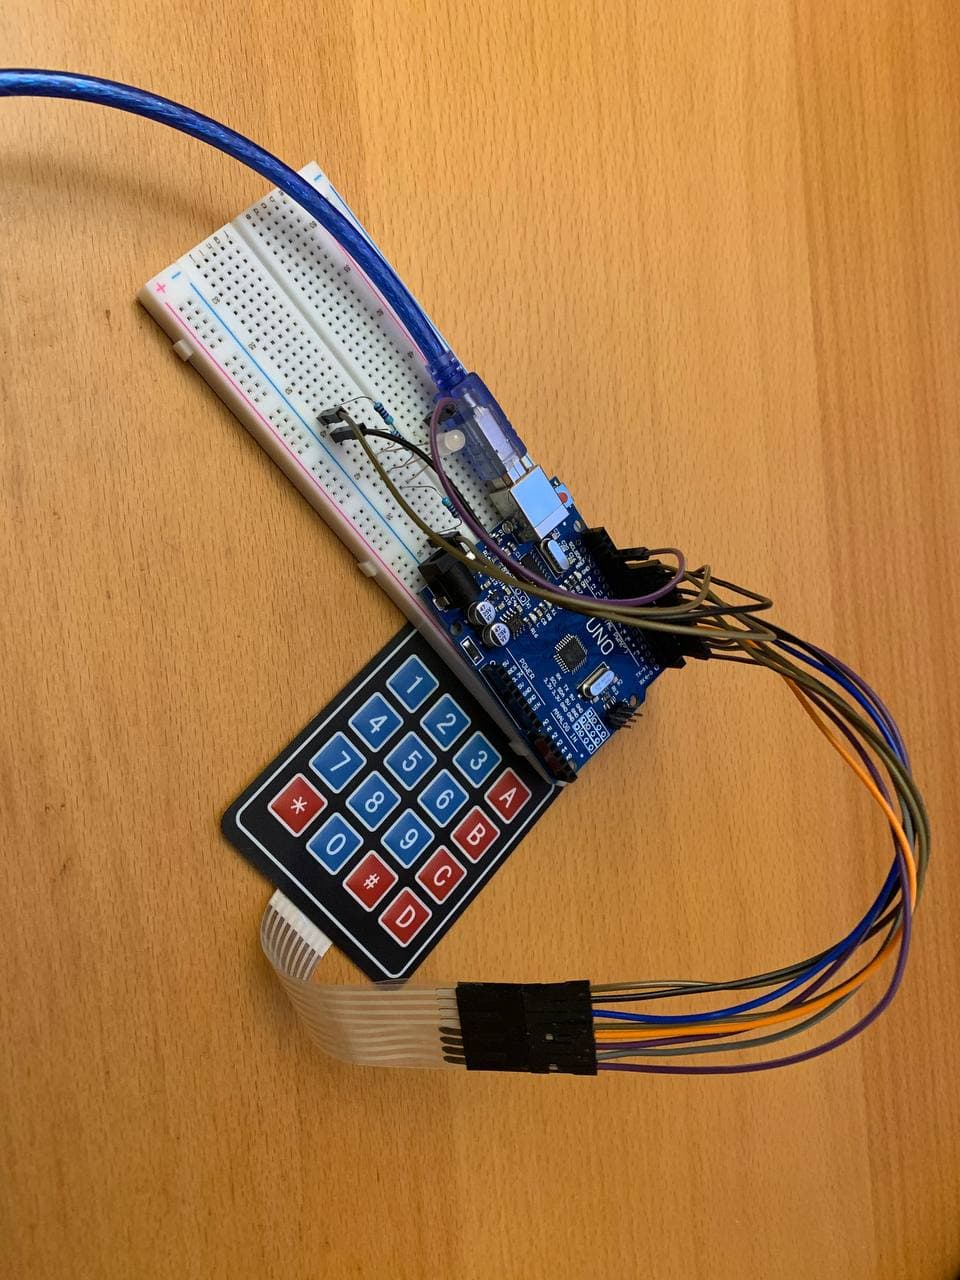
\includegraphics[width=0.6\textwidth]{images/picture.jpg}
    \label{fig:pic}
\end{figure}